\subsection{Переходная и весовая функции непрерывной системы. Свободная, вынужденная, переходная и установившаяся составляющие движения непрерывной системы}

\textit{Переходным процессом} называют процесс изменения во вреени различных переенных системы (фазовых, выходных, отклонений и т.д.) в ходе которых система изменяет свое состояние.
Перехдные процессы могут быть представлены аналитически или графически.
К графическим можно отнести: временные диаграммы переменных системы ($y(t), \dot y(t), \dots$) и фазовые траектории.
Для аналитического представления нужно режать ДУ системы.

Решение $y(t)$ (или $y_{\text{п}}(t)$~--- переходная составляющая) может быть представлено в виде суммы свободной и вынужденной составляющих:
\begin{equation}
    y(t) = y_{\text{св}}(t) + y_{\text{в}}(t)
\end{equation}
где $y_{\text{в}}(t)$~--- вынужденная составляющая, соответствующая переходному процессу системы при нулевых начальных условиях $y_0^{(i)} = 0$ и явлается реакцией системы на входное воздействие $u(t)$,
$y_{\text{св}} (t)$~--- свободная составляющая или переходный процесс автономной системы, соответствует решениям ОДУ системы и зависит от начальных условий.

Свободная составляющая зависит от полюсов системы и определяется выражениями:
\begin{enumerate}
    \item Для попарно различных (некратных) корней:
    \begin{equation}
        y_{\text{св}} (t) = \sum\limits_{i=0}^{n} y_i(t) = \sum\limits_{i=0}^{n} C_i e^{p_i t},
    \end{equation}
    где $C_i e^{p_t t}$~--- свободные колебания системы или моды.
    \begin{enumerate}
        \item Вещественные корни $p_i = \alpha_i$ представляют апериадичускую составляющую:
        \begin{equation}
            y_i = C_i e^{\alpha_i t}.
        \end{equation}
        \item Пары комплексно-сопряженных коней $p_i = \alpha_i \pm j \beta_i$ колебательную составляющую:
        \begin{equation}
            y_{i, i+1} = A_i e^{\alpha_i t} \sin{(\beta_i t + \phi_i)}.
        \end{equation}
    \end{enumerate}
    \item Для кратных корней:
    \begin{equation}
        y_{i, i+1} = (C_i + C_{i+1} t) \cdot e^{\alpha_i t}
    \end{equation}
\end{enumerate}

Вынужденная составляющая переходного процесса зависит от входного воздействия и может быть аналитически определена только для ряда частных случаев, соответствующих некоторым типовым входным сигналам. Наиболее распространнеными сигналами являеются единичный скачек, дельта-функция и гармоничческое воздействие.
\begin{enumerate}
    \item Единичный скачек.
    \begin{figure}[!h]
        \begin{minipage}[!h]{0.5\linewidth}
            \centering{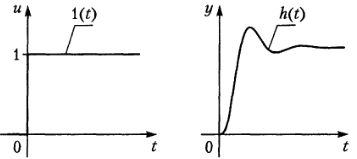
\includegraphics[width=0.8\linewidth]{images/input/1.png}}
        \end{minipage}
        \begin{minipage}[!h]{0.5\linewidth}
            \begin{equation}
                \mathbf{1}(t) = 
                \begin{cases}
                    0, for \: t \le 0, \\
                    1, for \: t > 0.
                \end{cases}
            \end{equation}
            Переходный процесс $y(t) = h(t)$ системы при ННУ и воздействии на ее вход ступенчатой единичной функции называется переходной функцией (характеристикой).
        \end{minipage}
    \end{figure}
    
    \item Дельта функция (единичная импульсная функция).
    \begin{figure}[!h]
        \begin{minipage}[!h]{0.5\linewidth}
            \centering{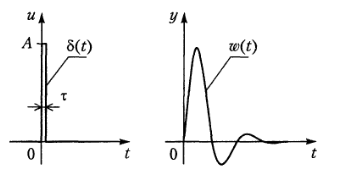
\includegraphics[width=0.8\linewidth]{images/input/delta.png}}
        \end{minipage}
        \begin{minipage}[!h]{0.5\linewidth}
            \begin{equation}
                \mathbf{\delta}(t) = \cfrac{d}{dt} \mathbf{1}(t).
            \end{equation}
            Переходный процесс $y(t) = w(t)$ системы при ННУ и воздействии на ее вход дельта-функции называется весовой функцией.
        \end{minipage}
    \end{figure}
\end{enumerate}

\textit{Установившейся режим}~--- это работа системы при $t \rightarrow \infty$:
\begin{equation}
    y_{\text{у}}(t) = \lim\limits_{t \rightarrow \infty} y_{\text{св}}(t)
    \quad\Rightarrow
    y(t) = y_{\text{п}}(t) + y_{\text{у}}(t)
\end{equation}

Если существуте предел (т.е. при достаточно больших t отсутствуют движения в системе)
\begin{equation}
    \lim\limits_{t \rightarrow \infty} y(t) = y_{\text{у}}(t),
\end{equation}
то такой режим называется статический режим работы системы.